\subsection{Ca sử dụng chia sẻ vị trí}
\noindent Ca sử dụng này mô tả cách người dùng chia sẻ vị trí thời gian thực của họ với các thành viên khác trong cùng một chuyến đi đang diễn ra. Tính năng này giúp các thành viên dễ dàng tìm thấy nhau hoặc theo dõi tiến trình di chuyển. Bảng~\ref{tab:uc_share_location_spec} trình bày chi tiết đặc tả ca sử dụng, bao gồm luồng sự kiện chính, luồng thay thế, các điều kiện và yêu cầu liên quan. Các biểu đồ hoạt động, quan hệ (Bảng~\ref{tab:uc_share_location_diagrams}) và tuần tự (Hình~\ref{fig:3-3-16-sequence-diagram}) minh họa rõ hơn về quy trình và tương tác hệ thống.
% \vspace{0.5cm} % Adjust spacing if needed

% Use longtable environment
% Need \usepackage{longtable} and \usepackage{calc} in preamble
\begin{longtable}{| p{4cm} | p{\dimexpr\linewidth-4cm-4\tabcolsep} |} % Adjust widths as needed
    \caption{Đặc tả ca sử dụng chia sẻ vị trí} % Caption inside longtable (no period)
    \label{tab:uc_share_location_spec} \\ % Label after caption

    \hline
    \textbf{Mô tả} & Người dùng trong cùng chuyến đi có thể chia sẻ vị trí khi chuyến đi đang diễn ra. \\
    \hline
    \endfirsthead % Header for the first page

    % No \endhead content needed

    % No \endfoot content needed

    \hline % Footer for the last page
    \endlastfoot

    % --- Table Content ---
    \textbf{Luồng cơ bản} & 1. Người dùng chọn một chuyến đi đang diễn ra. \newline
                           2. Hệ thống lấy dữ liệu chi tiết của chuyến đi và hiển thị. \newline
                           3. Người dùng bấm "Chia sẻ vị trí". \newline
                           4. Hệ thống điều hướng người dùng ra trang hiển thị bản đồ. \newline
                           5. Hệ thống yêu cầu quyền truy cập vị trí liên tục. \newline
                           6. Người dùng cấp quyền. \newline
                           7. Hệ thống cập nhật liên tục trong thời gian thực vị trí của bản thân người dùng và các người dùng khác tham gia chia sẻ vị trí trong chuyến đi. \\
    \hline
    \textbf{Luồng thay thế} & Nếu người dùng không cấp quyền truy cập vị trí, hệ thống sẽ không thể chia sẻ vị trí của họ và chỉ hiển thị vị trí của các thành viên khác (nếu có). \\
    \hline
    \textbf{Tiền điều kiện} & - Người dùng đang đăng nhập và phiên đăng nhập chưa kết thúc.\newline
                           - Người dùng đã tạo hoặc tham gia ít nhất một chuyến đi. \newline
                           - Chuyến đi đang trong trạng thái "Đang diễn ra". \\
    \hline
    \textbf{Hậu điều kiện} & - Hệ thống cập nhật vị trí của người dùng và các người dùng khác trong chuyến đi trên bản đồ thời gian thực. \newline
                           - Hệ thống tạo thông báo đẩy trong thiết bị để chạy nền tác vụ chia sẻ vị trí. \\
    \hline
    \textbf{Yêu cầu phi chức năng} & - Hệ thống cập nhật vị trí trên bản đồ với độ trễ dưới 5 giây. \newline
                                   - Tính năng chia sẻ vị trí cần tối ưu để không tiêu tốn quá nhiều pin thiết bị. \\
    % --- End Table Content ---

\end{longtable}
\vspace{0.8cm}

\begin{table}[H] % Wrap the diagrams table
    \centering
    \caption{Biểu đồ hoạt động và quan hệ ca sử dụng chia sẻ vị trí} % Add caption (no period)
    \label{tab:uc_share_location_diagrams} % Add label
    \begin{tabular}{| c | c |}
        \hline
        \textbf{Biểu đồ hoạt động} & \textbf{Quan hệ} \\
        \hline
        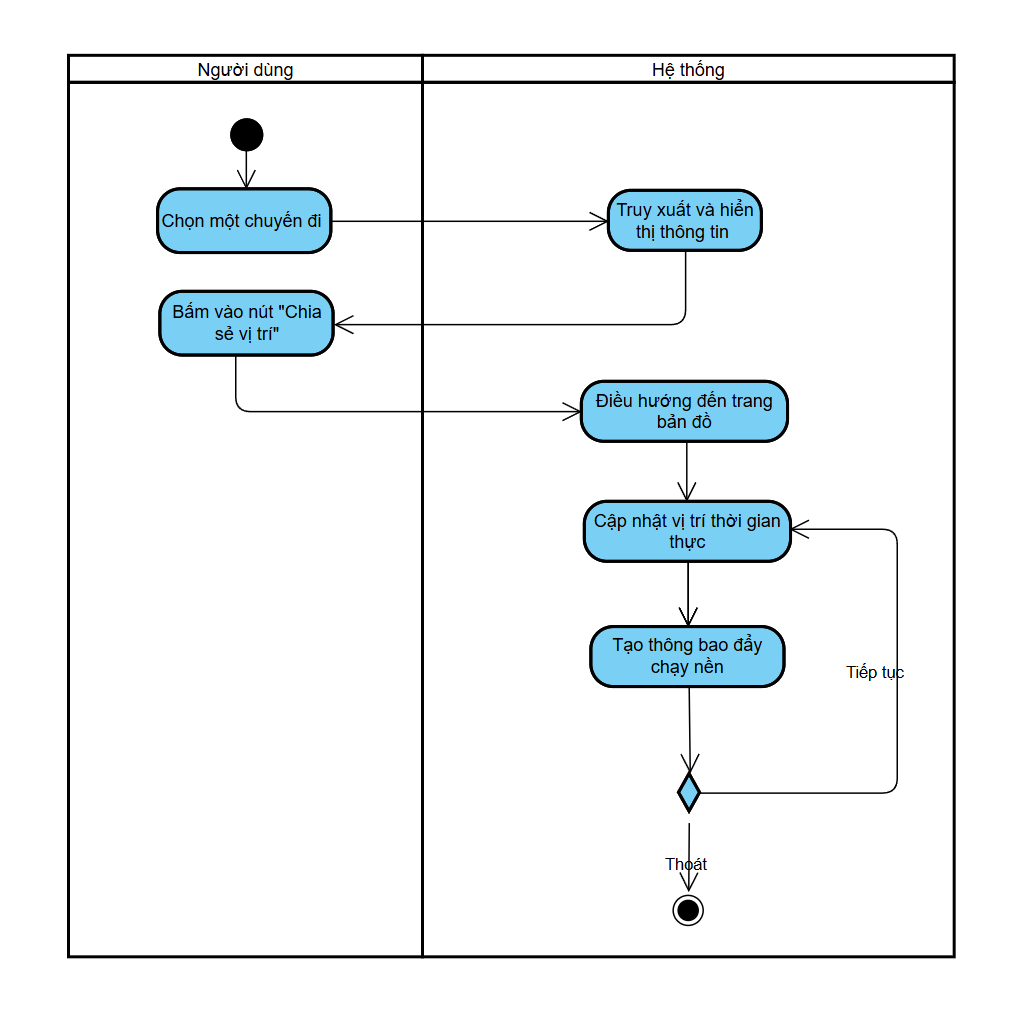
\includegraphics[width=0.5\linewidth]{figures/c3/3-3-16-ad.png} % Specified width
        &
        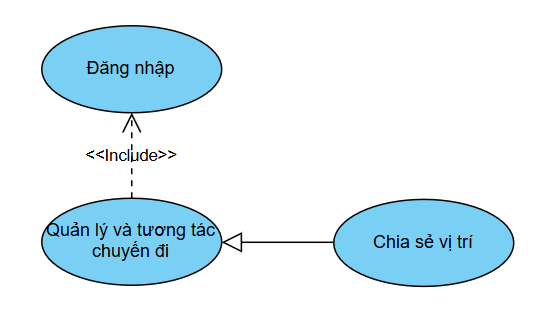
\includegraphics[width=0.45\linewidth]{figures/c3/3-3-16-rd.png} \\ % Specified width
        \hline
    \end{tabular}
\end{table}

\begin{figure}[H]
    \centering
    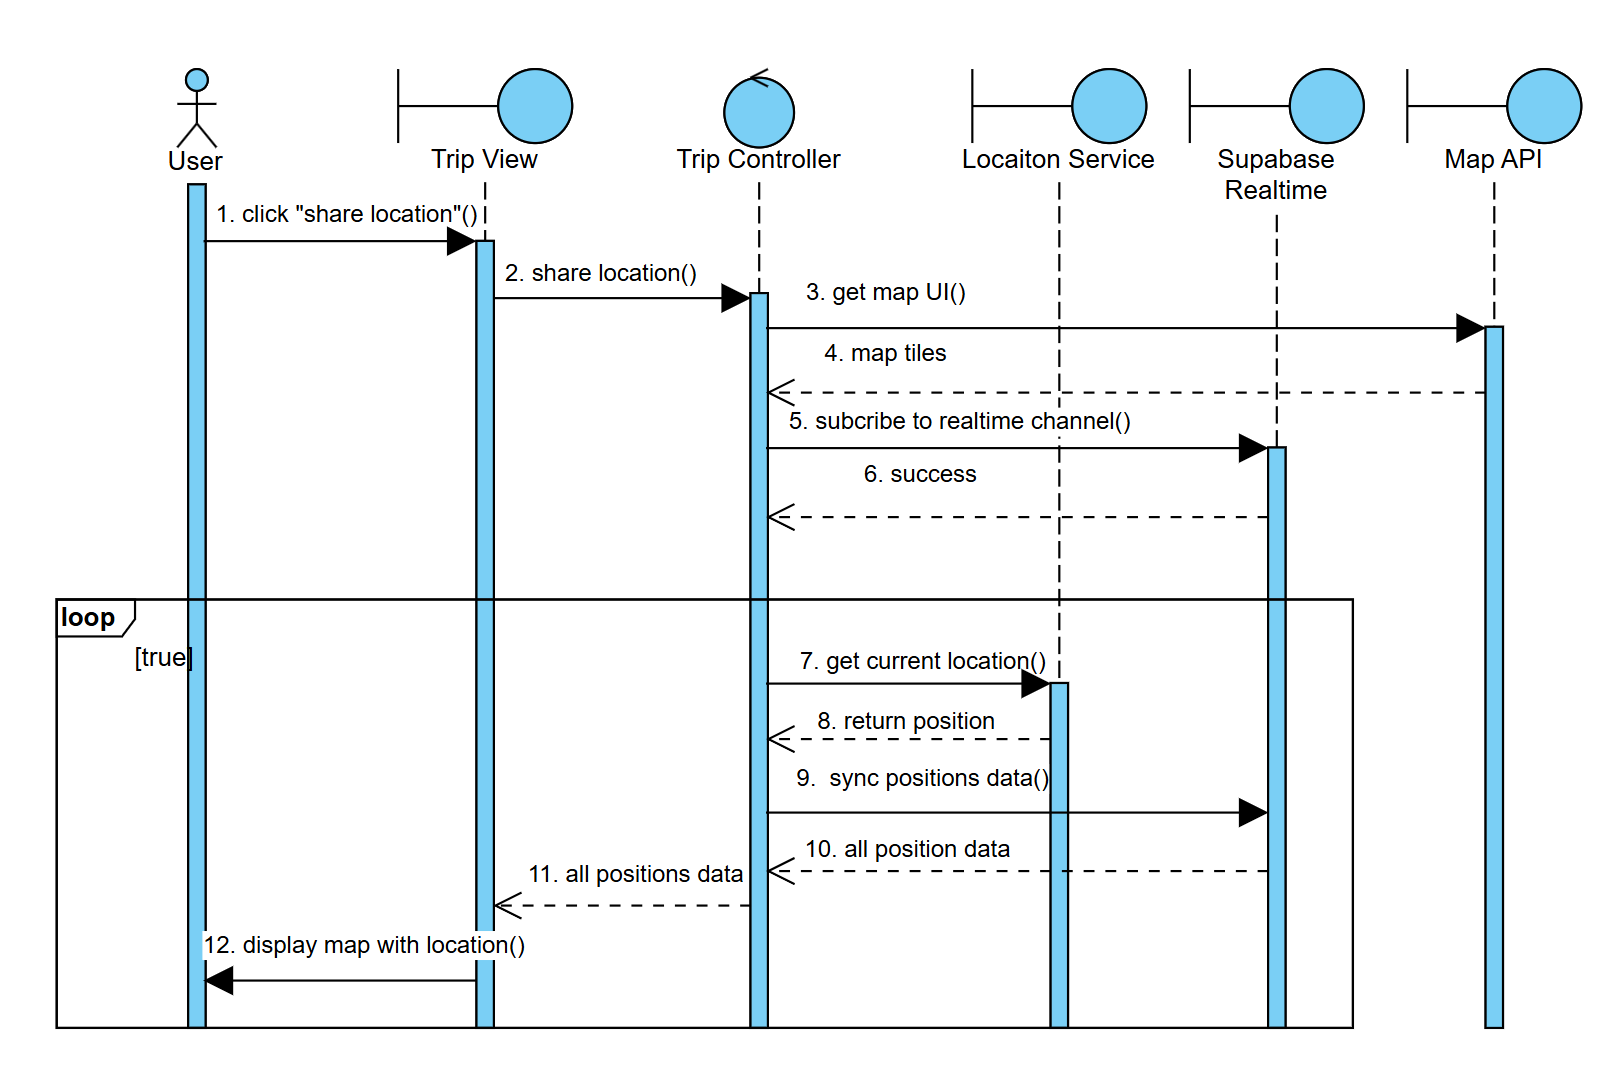
\includegraphics[width=1\textwidth]{figures/c3/3-3-16-sd.png} % Specified width
    \caption{Biểu đồ tuần tự ca sử dụng chia sẻ vị trí} % (no period)
    \label{fig:3-3-16-sequence-diagram}
\end{figure}